\documentclass[11pt,titlepage]{article}
\usepackage[parfill]{parskip}
\usepackage{textcomp}
\usepackage{fullpage}
\usepackage{amsmath}
\usepackage{amssymb}
\usepackage{gensymb}
\usepackage{color}
\usepackage{graphicx}
\graphicspath{ {images/} }
\usepackage{float}
\restylefloat{table}
\usepackage{array}

\author{Rane Brown \\ Brian Douglass}
\title{ECEN 4593: Memory Simulation Project}
\date{\today}

\begin{document}
\maketitle
\tableofcontents
\listoffigures \listoftables
\newpage

\section{Introduction}
This project simulates a two level cache using the C programming language. The memory hierarchy consists of a L1 instruction cache, a L1 data cache and a unified L2 cache. In addition, each cache level has a victim cache which is setup as an eight deep fully associative cache. If there is a miss at a particular cache level then that level's victim cache is checked before making a request to the next level in the hierarchy. The caches are \emph{write-allocate}, \emph{write-back} caches which means a dirty bit must be used to track when a write request occurs. Each cache maintains a LRU (least recently used) replacement policy for each set in a set associative cache or in a fully associative cache. This project evaluates the performance of nine different memory configurations using sample traces from a selection of six SPEC benchmarks. The bus widths, transfer times, hit/miss times, and various other important parameters can be found in the official project description.

\section{Setup and Code Structure}
When a simulation is executed, the cache first needs to be structured and built. The structure of the cache is determined from a configuration file passed in at startup. This file contains the cache size and number of ways for all of the cache levels and stores it in a structure on the heap. From there, an array of pointers to linked lists is built. The length of the array is the number of levels in the cache, and the number of ways for the cache level determines the number of nodes (i.e. an L1 4-way cache has four nodes at each index, a direct mapped has a single node per index and the fully associative has one index and $[cache size / block size]$ nodes).

After configuration and setup the lines from the trace are read in and parsed. After some initial information is gathered the necessary addressing information is collected and sent to the corresponding L1 cache search function. After checking the L1, the program calls a function that will initiate a check of the L1 victim cache, L2 cache, and L2 victim cache returning only when a hit occurs. If a hit occurs at any level of a cache, the proper blocks are swapped as necessary. When swapping, only the values in each node is swapped, the actual nodes are kept in their own cache level. When new blocks are brought in, the node is "bumped" to the from of the list. In doing this an LRU policy is maintained with the least recent block at the end of every list.

Upon completion of the trace read, the important calculations are made and the results are printed to the Simulation Results page for that trace and configuration. All simulation results files are included in this report in the Appendix section. A complete copy of the code is also included in the Appendix section in a Doxygen generated file. In addition to the code for this project, the Doxygen report includes information about all functions and structures used.

\section{Performance Evaluation}
In evaluating the performance of the different cache configurations the natural place to begin is in an analysis of the Clock cycles Per Instruction (CPI) for each trace.  In this first section, the CPI is examined to find any patterns, and then those patterns are investigated to determine what causes them. It should be noted that the plots in this section that show the hit/miss rates for each cache level use a $log_{10}$ scale. This was necessary because the hit rates are much larger numbers than the miss rates and without scaling the data a useful plot cannot be created.
    \subsection{astar}
    Figure \ref{fig:CPIastar} shows the different CPI values for each cache configuration while running the astar trace. The interesting observation from this graph are the five configurations that give the same CPI. Each of these configurations have a direct-mapped L2 cache, changing only the associativity of the L1 cache. As soon as the L2 associativity is increased, the CPI begins to decrease as expected, with the fully-associative configuration providing the best CPI. Another contributing factor to this relatively consistent CPI can be seen from the low miss rate in the L1 instruction cache.
     \begin{figure}[H]
          \centering
          \begin{minipage}{.5\textwidth}
            \centering
            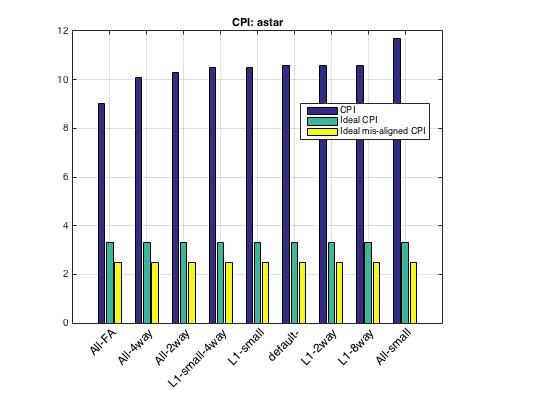
\includegraphics[width=9cm]{CPIastar}
            \caption{CPI: astar}
            \label{fig:CPIastar}
          \end{minipage}%
          \begin{minipage}{.5\textwidth}
            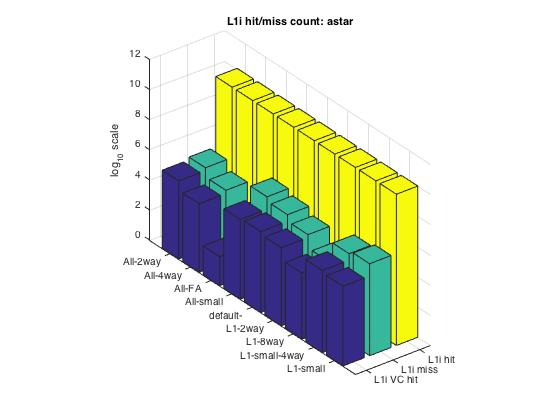
\includegraphics[width=9cm]{L1IHM_astar}
            \caption{L1 Inst. Cache hits/misses: astar}
            \label{fig:L1IHM_astar}
          \end{minipage}%
    \end{figure}
        \begin{figure}[H]
          \centering
          \begin{minipage}{.45\textwidth}
            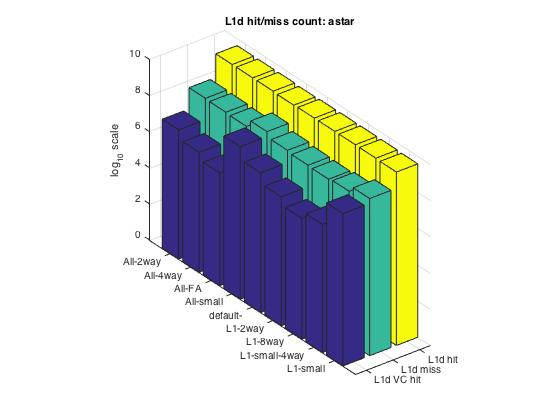
\includegraphics[width=9cm]{L1DHM_astar}
            \caption{L1 Data Cache hits/misses: astar}
            \label{fig:L1DHM_astar}
          \end{minipage}
          \begin{minipage}{.45\textwidth}
            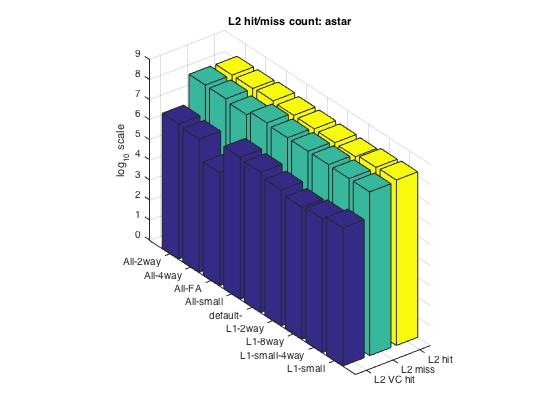
\includegraphics[width=9cm]{L2HM_astar}
            \caption{L2 Cache hits/misses: astar}
            \label{fig:L2HM_astar}
          \end{minipage}
    \end{figure}

    \subsection{bzip2}
    Figure \ref{fig:CPIbzip2} which shows the CPI values from the bzip2 traces, gives little in the way of a pattern or comparison between different cache configurations. The interesting part of this simulation can be seen by comparing the bzip2 CPI's to other trace results. The difference can be seen in Figure \ref{fig:L1IHM_bzip2}, which shows L1 instruction cache hits and misses. Here we can see a lower than usual miss count, and a high hit count. This, and the libquantum trace simulations shown in Figure \ref{fig:L1IHM_bzip2} shows again that a direct-mapped configuration produces lower performance than almost any level of higher associativity.
        \begin{figure}[H]
          \centering
          \begin{minipage}{.5\textwidth}
            \centering
            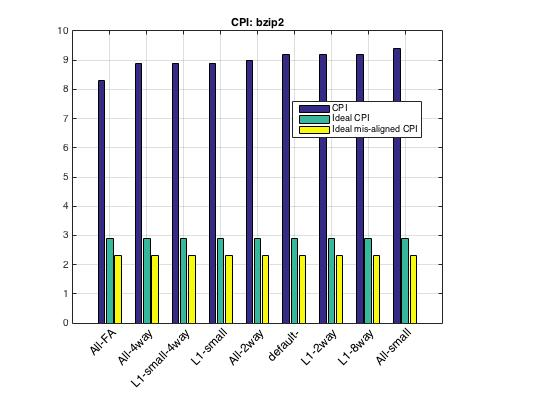
\includegraphics[width=10cm]{CPIbzip2}
            \caption{CPI: bzip2}
            \label{fig:CPIbzip2}
          \end{minipage}%
          \begin{minipage}{.5\textwidth}
            \centering
            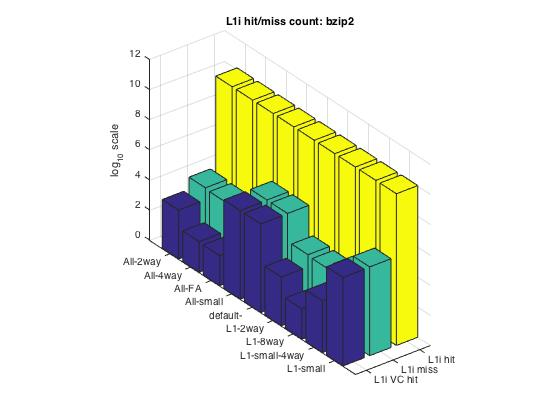
\includegraphics[width=10cm]{L1IHM_bzip2}
            \caption{L1 Inst. Cache hits/misses: bzip2}
            \label{fig:L1IHM_bzip2}
          \end{minipage}%
        \end{figure}

    \subsection{gobmk}
    The gobmk simulation was the first simulation to provide a clear look at how increasing the associativity (as well as the size for similar associativity) increases the performance and decreases the CPI of each simulation. These results are the anticipated outcome for general CPU caching, the larger the cache and higher the number of associativity, the better the performance. Looking at the hit and miss counts for each of the caches, (shown in Figures \ref{fig:L1IHM_gobmk}, \ref{fig:L1DHM_gobmk}, and, \ref{fig:L2HM_gobmk}) there are relatively consistent and higher miss counts at every level. These counts are the contributing factors to the CPI values calculated.
    \begin{figure}[H]
          \centering
          \begin{minipage}{.5\textwidth}
            \centering
            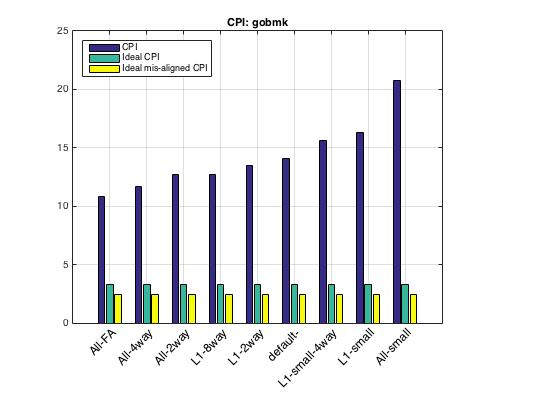
\includegraphics[width=9cm]{CPIgobmk}
            \caption{CPI: gobmk}
            \label{fig:CPIgobmk}
          \end{minipage}%
          \begin{minipage}{.5\textwidth}
            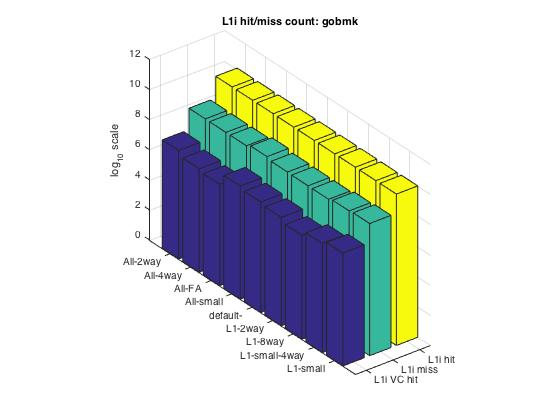
\includegraphics[width=9cm]{L1IHM_gobmk}
            \caption{L1 Inst. Cache hits/misses: gobmk}
            \label{fig:L1IHM_gobmk}
          \end{minipage}%
    \end{figure}
        \begin{figure}[H]
          \centering
          \begin{minipage}{.45\textwidth}
            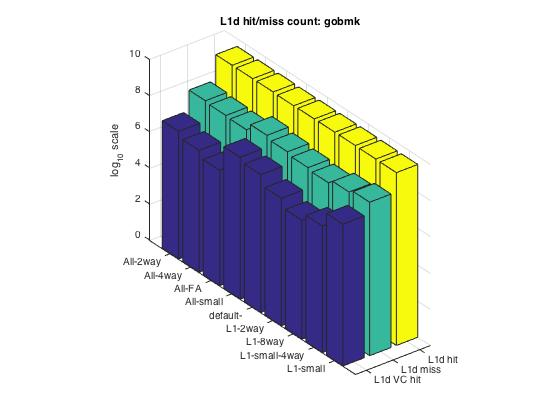
\includegraphics[width=9cm]{L1DHM_gobmk}
            \caption{L1 Data Cache hits/misses: gobmk}
            \label{fig:L1DHM_gobmk}
          \end{minipage}
          \begin{minipage}{.45\textwidth}
            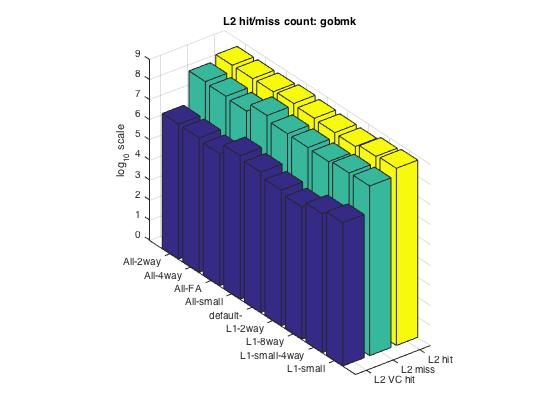
\includegraphics[width=9cm]{L2HM_gobmk}
            \caption{L2 Cache hits/misses: gobmk}
            \label{fig:L2HM_gobmk}
          \end{minipage}
    \end{figure}

    \subsection{libquantum}
    The libquantum trace simulation returned results similar to those of the bzip2 trace, however more extreme. Figure \ref{fig:CPIlibquantum} shows identical CPI's for each configuration. This is again curious until the hit/miss graph shown in Figure \ref{fig:L1IHM_libquantum} is examined. Here we see  a \emph{very} low miss count for each of the cache configurations. This is evident of either a small set of instructions being used, or very high locality in the libquantum trace.
        \begin{figure}[H]
          \centering
          \begin{minipage}{.45\textwidth}
             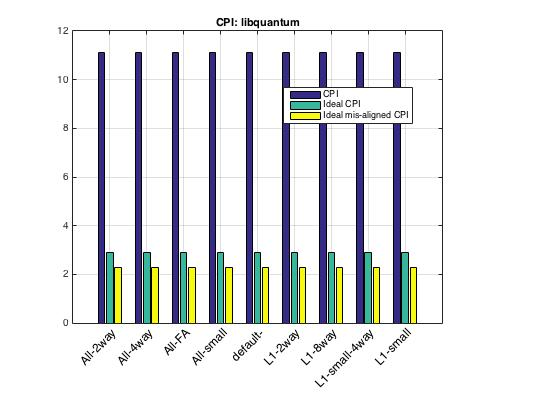
\includegraphics[width=9cm]{CPIlibquantum}
             \caption{CPI: libquantum}
             \label{fig:CPIlibquantum}
          \end{minipage}
          \begin{minipage}{.45\textwidth}
              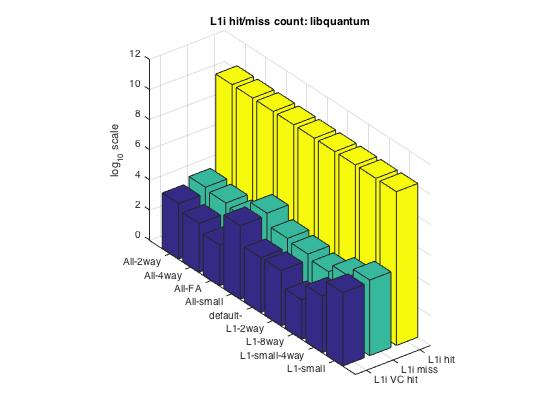
\includegraphics[width=9cm]{L1IHM_libquantum}
              \caption{L1i hits/misses: libquantum}
              \label{fig:L1IHM_libquantum}
          \end{minipage}%
          \end{figure}
          \begin{figure}[H]
          \centering
          \begin{minipage}{.45\textwidth}
               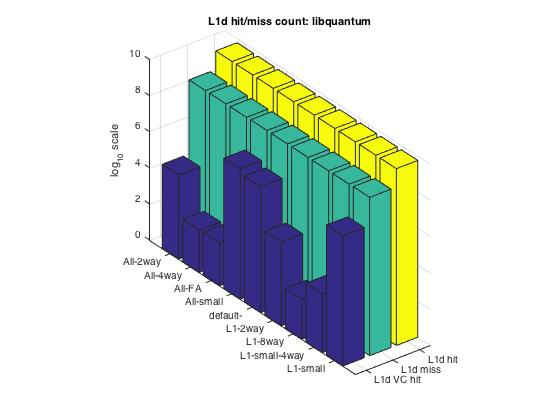
\includegraphics[width=9cm]{L1DHM_libquantum}
               \caption{L1d hits/misses: libquantum}
               \label{fig:L1DHM_libquantum}
          \end{minipage}
          \begin{minipage}{.45\textwidth}
               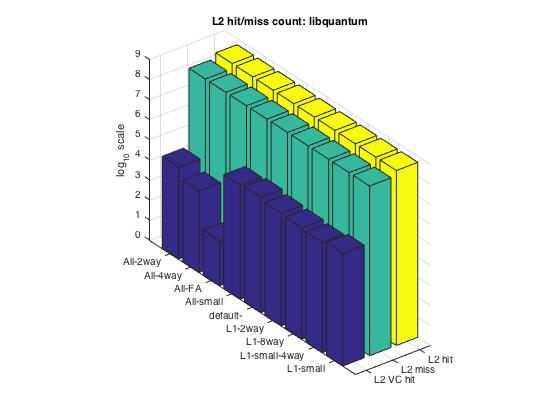
\includegraphics[width=9cm]{L2HM_libquantum}
               \caption{L2 hits/misses: libquantum}
               \label{fig:L2HM_libquantum}
          \end{minipage}
        \end{figure}

    \subsection{omnetpp}
    The omnetpp simulation shows data very much like that of the gobmk. We see a high miss count and the corresponding CPI improvement as the associativity and cache size increases.
    \begin{figure}[H]
      \centering
      \begin{minipage}{.45\textwidth}
      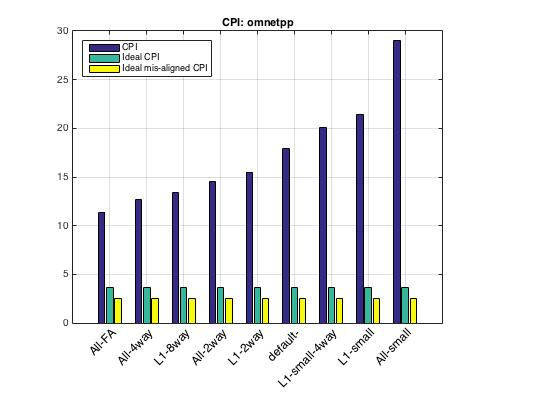
\includegraphics[width=9cm]{CPIomnetpp}
      \caption{CPI: omnetpp}
      \label{fig:CPIomnetpp}
      \end{minipage}
      \begin{minipage}{.45\textwidth}
            \centering
            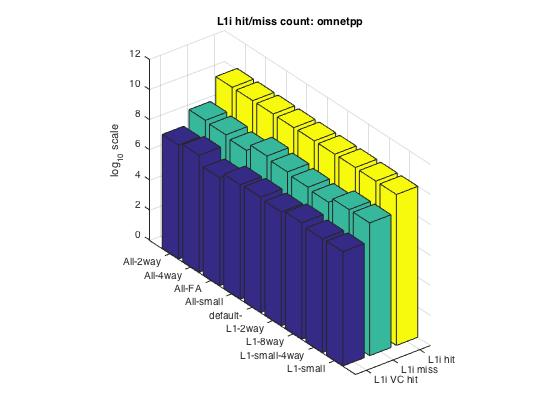
\includegraphics[width=9cm]{L1IHM_omnetpp}
            \caption{L1i hits/misses: omnetpp}
            \label{fig:L1IHM_omnetpp}
          \end{minipage}%
           \end{figure}
          \begin{figure}[H]
          \centering
          \begin{minipage}{.45\textwidth}
            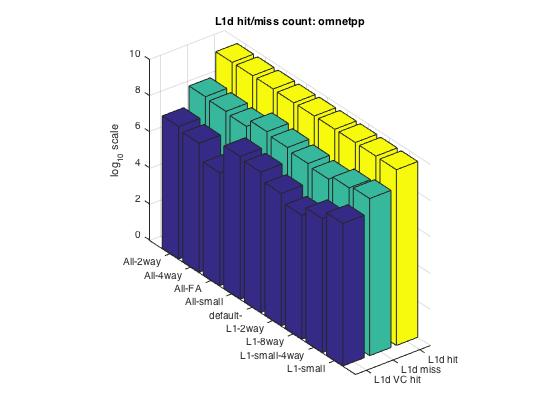
\includegraphics[width=9cm]{L1DHM_omnetpp}
            \caption{L1i hits/misses: omnetpp}
            \label{fig:L1DHM_omnetpp}
          \end{minipage}
          \begin{minipage}{.45\textwidth}
            \centering
            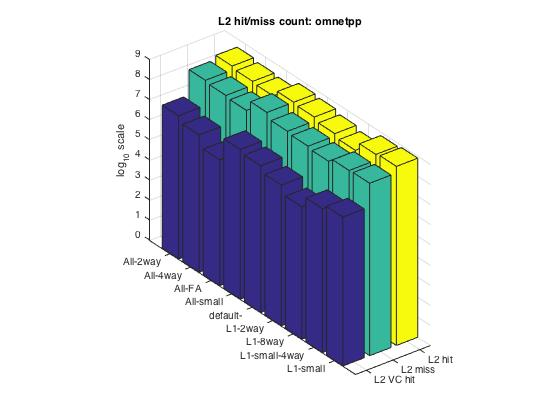
\includegraphics[width=9cm]{L2HM_omnetpp}
            \caption{L2 hits/misses: omnetpp}
            \label{fig:L2HM_omnetpp}
          \end{minipage}
    \end{figure}

    \subsection{sjeng}
    The final simulation is the sjeng and this trace follows the same pattern as gobmk and omnetpp. Again, we see higher miss counts in all levels of the memory and consistent improvements to the CPI as the size and associativities increase.
        \begin{figure}[H]
      \centering
      \begin{minipage}{.45\textwidth}
      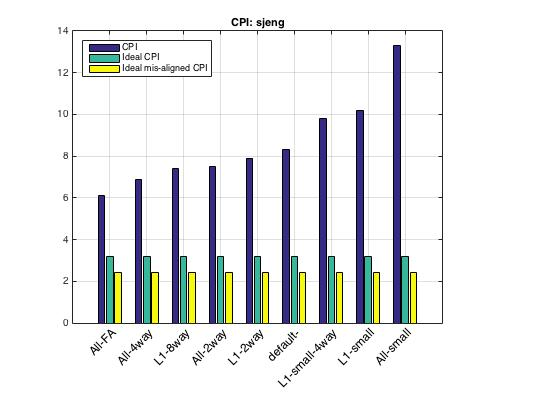
\includegraphics[width=9cm]{CPIsjeng}
      \caption{CPI: sjeng}
      \label{fig:CPIsjeng}
      \end{minipage}
      \begin{minipage}{.45\textwidth}
            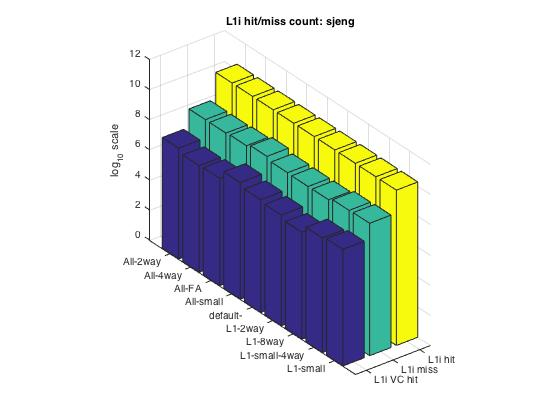
\includegraphics[width=9cm]{L1IHM_sjeng}
            \caption{L1 Inst. Cache hits/misses: sjeng}
            \label{fig:L1IHM_sjeng}
          \end{minipage}%
           \end{figure}
          \begin{figure}[H]
          \centering
          \begin{minipage}{.45\textwidth}
            \centering
            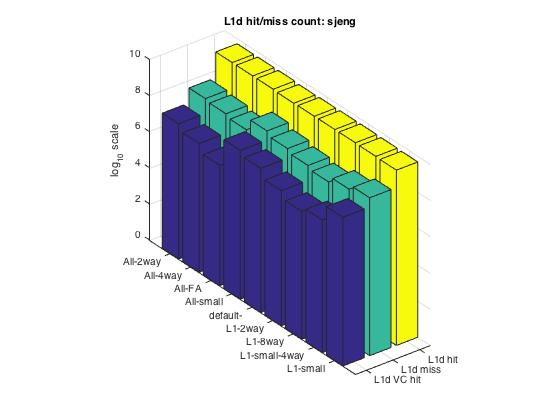
\includegraphics[width=9cm]{L1DHM_sjeng}
            \caption{L1 Data Cache hits/misses:sjeng}
            \label{fig:L1DHM_sjeng}
          \end{minipage}
          \begin{minipage}{.45\textwidth}
            \centering
            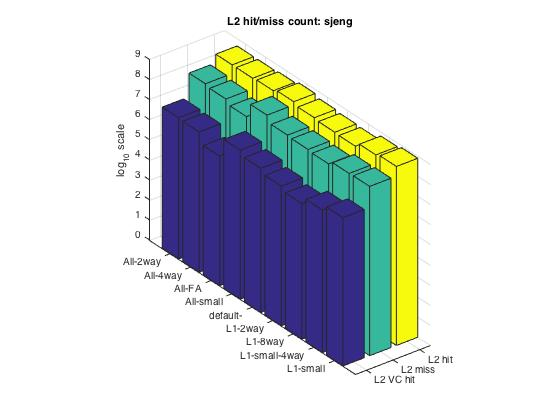
\includegraphics[width=9cm]{L2HM_sjeng}
            \caption{L2 Cache hits/misses: sjeng}
            \label{fig:L2HM_sjeng}
          \end{minipage}
    \end{figure}
\pagebreak
    \section{Overall Performance Comparison}
    From the previous performance evaluations, two major patterns emerge. First, for traces with high locality in the instruction list, we see similar CPI's across the range of different configurations. Traces such as the libquantum, which show a very low miss count in the L1 cache have an identical CPI for each cache scheme. Compare that to the gobmk trace which shows a high miss count at all levels of cache, and a wide range of CPI values are found. This leads to the second pattern, that the higher the miss count in the caches, the more the architecture of the cache plays a role in performance. This role shows that the higher the associativity of a cache, the better the performance. If two caches have the same associativity, then the larger cache shows the better performance. For example, the omnetpp trace received an almost 300\% improvement to its CPI going between the All-small direct-mapped and the All-FA cache configurations.
     \begin{figure}[H]
      \centering
      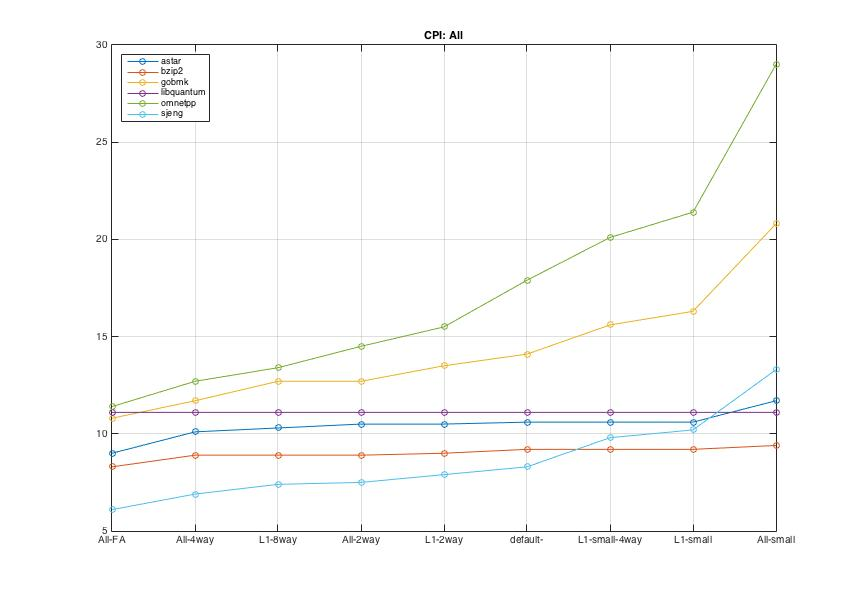
\includegraphics[scale=0.45]{CPIall}
      \caption{CPI comparison}
      \label{fig:CPIall}
    \end{figure}
     \begin{figure}[H]
      \centering
      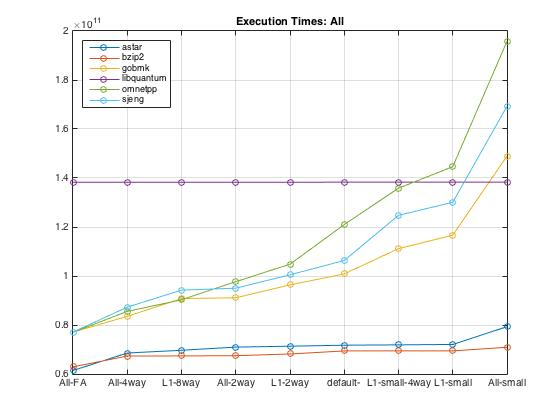
\includegraphics[scale=0.65]{ExecutionTimes_All}
      \caption{Execution Time comparison}
      \label{fig:etalll}
    \end{figure}

    Viewing the executions times of a simulation for different configurations is useful but it is also helpful to compare the actual execution times to the ideal case. In the ideal case there would be 100\% hit rate in the L1 cache. There are two ideal cases to consider: first, the bus width between the processor and the L1 cache is as wide as necessary to accommodate the number of bytes in the request; second, the bus between the processor and the L2 cache is 4 bytes. In the second scenario it is possible for a trace to require multiple accesses to the L1 cache since the memory addresses must align on 4 byte boundaries. Plots \ref{fig:idealA} -- \ref{fig:idealS} show the relation between the actual execution time for each configuration versus the two ideal cases. Also, table \ref{tbl:ideal} shows how much faster the ideal and ideal mis-aligned execution is than the actual execution time. These values are averaged across all configurations for a given trace.
    \begin{figure}[H]
      \centering
      \begin{minipage}{.5\textwidth}
        \centering
        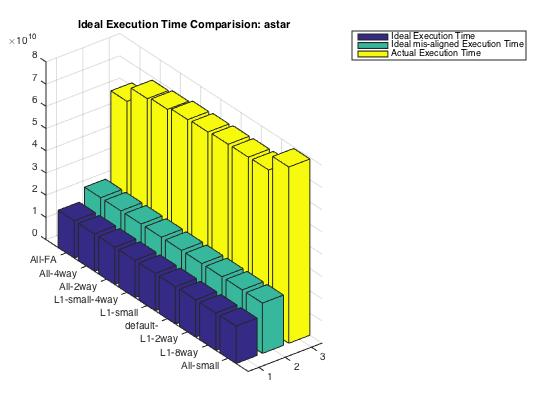
\includegraphics[width=10cm]{idealAstar}
        \caption{Ideal Execution Times: astar}
        \label{fig:idealA}
      \end{minipage}%
      \begin{minipage}{.5\textwidth}
        \centering
        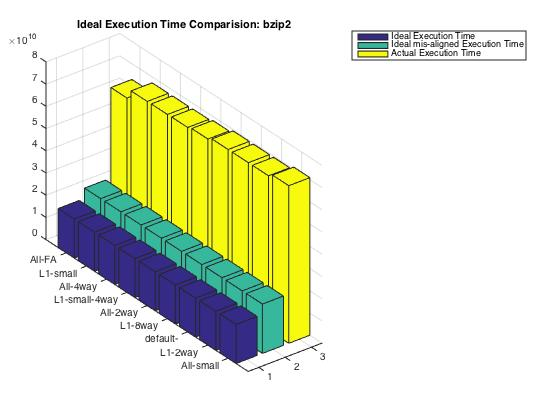
\includegraphics[width=10cm]{idealBzip2}
        \caption{Ideal Execution Times: bzip2}
        \label{fig:idealB}
      \end{minipage}
    \end{figure}
    \begin{figure}[H]
      \centering
      \begin{minipage}{.5\textwidth}
        \centering
        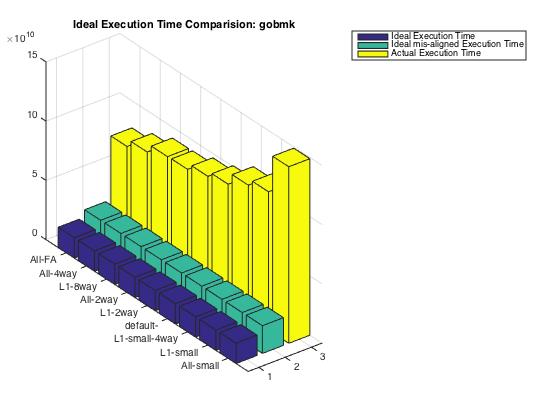
\includegraphics[width=10cm]{idealGobmk}
        \caption{Ideal Execution Times: gobmk}
        \label{fig:idealG}
      \end{minipage}%
      \begin{minipage}{.5\textwidth}
        \centering
        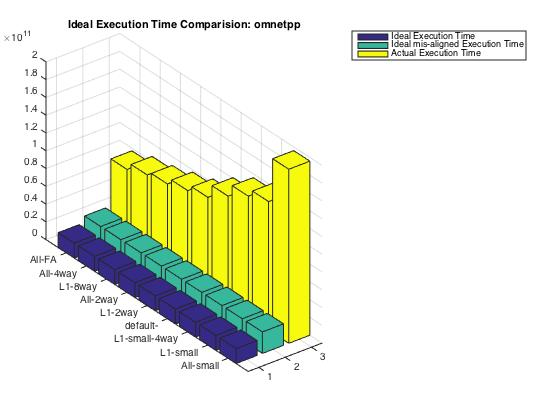
\includegraphics[width=10cm]{idealOmnetpp}
        \caption{Ideal Execution Times: omnetpp}
        \label{fig:idealO}
      \end{minipage}
    \end{figure}
    \begin{figure}[H]
      \centering
      \begin{minipage}{.5\textwidth}
        \centering
        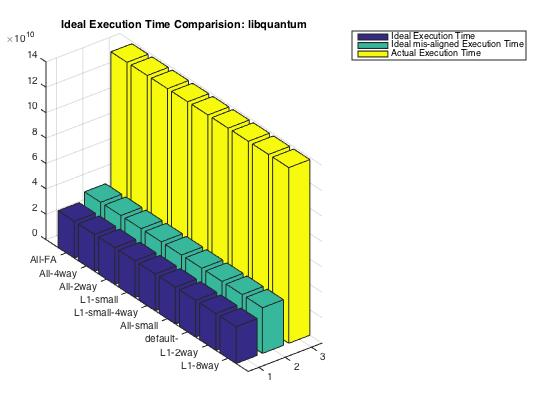
\includegraphics[width=10cm]{idealLibquantum}
        \caption{Ideal Execution Times: libquantum}
        \label{fig:idealL}
      \end{minipage}%
      \begin{minipage}{.5\textwidth}
        \centering
        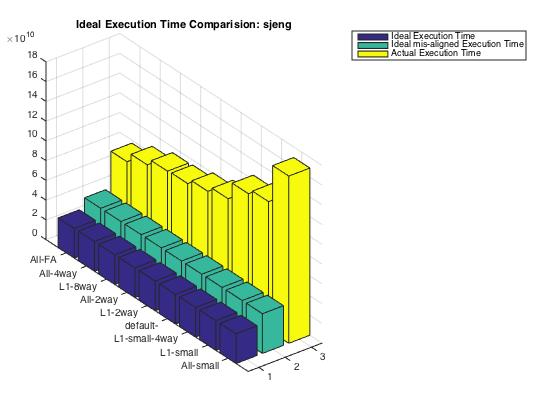
\includegraphics[width=10cm]{idealSjeng}
        \caption{Ideal Execution Times: sjeng}
        \label{fig:idealS}
      \end{minipage}
    \end{figure}

    \begin{table}[H]
      \centering
      \begin{tabular}{|m{4cm}|m{4cm}|m{4cm}|}
        \hline
        Trace & Ideal & Ideal mis-aligned \\
        \hline
        astar & 4.2150 & 3.1272 \\
        \hline
        bzip2 & 3.8738 & 3.0652 \\
        \hline
        gobmk & 5.9394 & 4.3599 \\
        \hline
        omnetpp & 6.9832 & 4.8438 \\
        \hline
        libquantum & 4.7694 & 3.8467 \\
        \hline
        sjeng &  3.6417 & 2.7240 \\
        \hline
      \end{tabular}
      \caption{Speedup: Ideal Cases} \label{tbl:ideal}
    \end{table}

\section{Cost Evaluation}
An additional method used to evaluate the different cache configurations is to look at the cost associated with a particular configuration. The costs are evaluated based on the following information:
\begin{itemize}
\item L1 cache
  \begin{itemize}
  \item \$100 for each 4KB
  \item \$100 for each doubling in associativity beyond direct-mapped
  \end{itemize}
\item L2 cache
  \begin{itemize}
  \item \$50 per 16KB
  \item \$50 for each doubling in associativity beyond direct-mapped
  \end{itemize}
\item Main memory
  \begin{itemize}
  \item base latency of 50 costs \$50
  \item base 8-byte mem chunk-size bandwidth costs \$25
  \item \$100 to increase the bandwidth (mem chunk-size) by a factor
    of 2
  \end{itemize}
\end{itemize}

\subsection{Cost by configuration}
Figure \ref{fig:totCost} shows the breakdown of the memory cost for each of the different configurations. The overall cost is shown as well as the cost for each level in the memory hierarchy. This plot shows that the All-small configuration results in the lowest cost while the All-FA (fully associative) configuration results in the highest cost. Section \ref{sec:costVperf} examines the relation between cost and performance.
\begin{figure}[H]
  \centering
  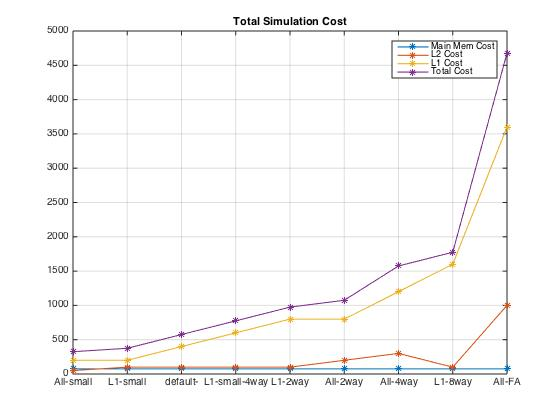
\includegraphics[scale=0.75]{totalCost}
  \caption{Cost by configuration}
  \label{fig:totCost}
\end{figure}

\subsection{Cost versus Performance} \label{sec:costVperf} The following series of bar graphs (figures \ref{fig:cvpastar}-\ref{fig:cvpsjeng}) displays the CPI versus cost for each trace and configuration. The values for the cost are divided by 100 and then the data is normalized between 0-1. This was necessary in order to display the large values of cost with the relatively lower values of CPI. Each plot is sorted with the best performance (shown in yellow) on the left. The cost associated with that performance level is represented in blue next to the CPI value. Clearly, the best performance is given by the fully associative configuration but this option also results in the highest cost. A better choice would be to use these plots and select the lowest CPI with the correspondingly lowest cost. The best option is somewhat subjective and related to the budget available when designing the cache but the All-2way configuration provides a decently low CPI while still maintaining a low cost.
\begin{figure}[H]
  \centering
  \begin{minipage}{.5\textwidth}
    \centering
    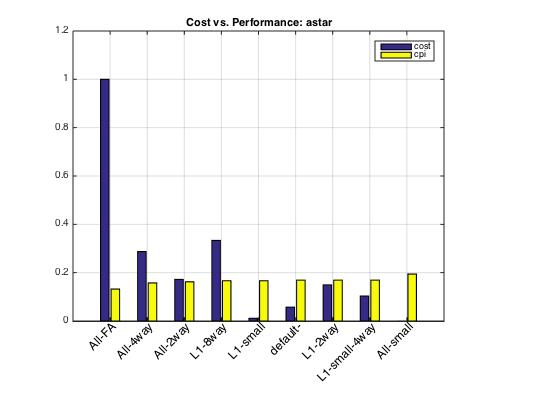
\includegraphics[width=10cm]{cvpastar}
    \caption{Cost vs. CPI astar}
    \label{fig:cvpastar}
  \end{minipage}%
  \begin{minipage}{.5\textwidth}
    \centering
    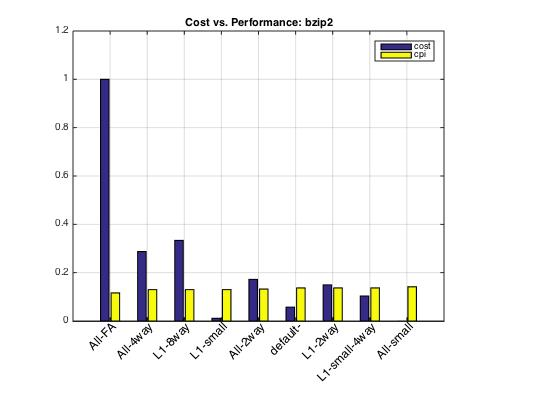
\includegraphics[width=10cm]{cvpbzip2}
    \caption{Cost vs. CPI bzip2}
    \label{fig:cvpbzip2}
  \end{minipage}
\end{figure}
\begin{figure}[H]
  \centering
  \begin{minipage}{.5\textwidth}
    \centering
    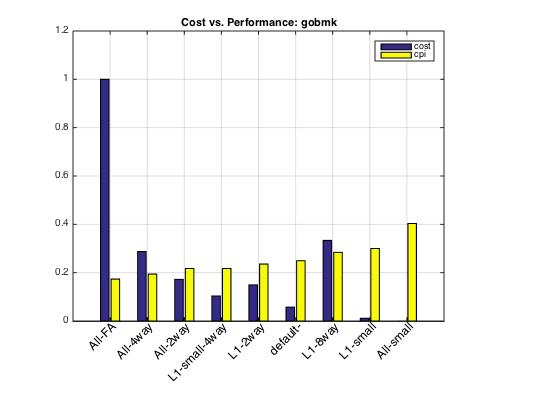
\includegraphics[width=10cm]{cvpgobmk}
    \caption{Cost vs. CPI gobmk}
    \label{fig:cvpgobmk}
  \end{minipage}%
  \begin{minipage}{.5\textwidth}
    \centering
    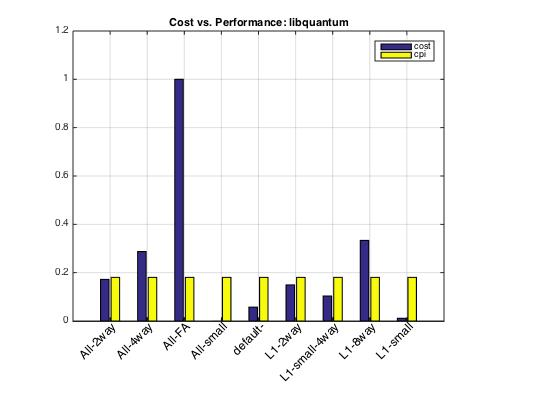
\includegraphics[width=10cm]{cvplibquantum}
    \caption{Cost vs. CPI libquantum}
    \label{fig:cvplibquantum}
  \end{minipage}
\end{figure}
\begin{figure}[H]
  \centering
  \begin{minipage}{.5\textwidth}
    \centering
    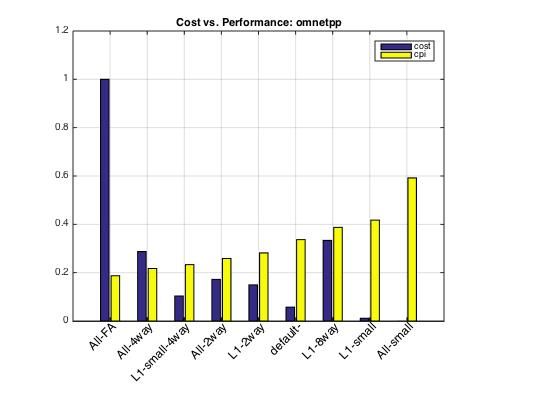
\includegraphics[width=10cm]{cvpomnetpp}
    \caption{Cost vs. CPI omnetpp}
    \label{fig:cvomnetpp}
  \end{minipage}%
  \begin{minipage}{.5\textwidth}
    \centering
    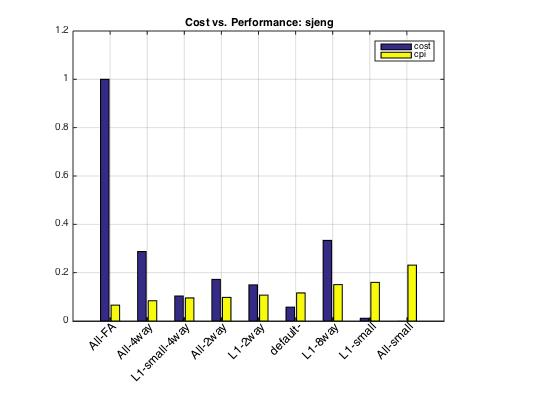
\includegraphics[width=10cm]{cvpsjeng}
    \caption{Cost vs. CPI sjeng}
    \label{fig:cvpsjeng}
  \end{minipage}
\end{figure}

\section{Main Memory Bandwidth Increase}
A method that can be used to increase the memory system performance is to increase the bandwidth to main memory. The base configuration uses a mem chunk-size of 8 bytes. Increasing this value will speed up each access to main memory. To evaluate the performance gains when the bandwidth is increased we ran three additional simulations using the sjeng trace. Each additional simulation used the default configuration with the bandwidth to main memory increasing from the default 8 bytes to 16, 32, and 64 bytes. The increase in bandwidth results in an associated increase in cost of \$100 for each doubling of mem chunk-size. Figure \ref{fig:exSj} displays the CPI versus cost using the same method described in section \ref{sec:costVperf}. It can be seen that the increasing the bandwidth to 64 bytes results in the lowest CPI of 6.3 but the cost is the highest. The base cost with a bandwidth of 8 bytes if \$575 and increasing the bandwidth to 64 bytes results in a cost of \$875. The cost increase of \$300 is fairly low and the CPI is reduced from 8.3 to 6.3. Our analysis it that accepting the additional cost to increase the bandwidth to 64 bytes is an acceptable compromise to realize a 25\% decrease in CPI.
\begin{figure}[H]
  \centering
  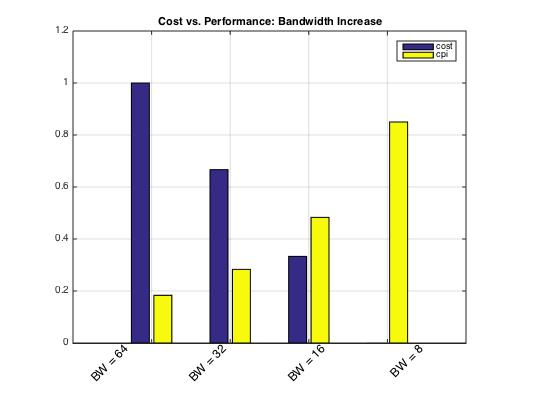
\includegraphics[scale=0.75]{extraSjeng}
  \caption{Cost vs. Performance: Bandwidth Increase}
  \label{fig:exSj}
\end{figure}

\section{Conclusion}
Overall, the memory simulator project was a success. Building the simulator provided us with a much greater understanding of how a cache works and how different configurations affect performance and cost. There are multiple choices that must be considered before implementing a memory hierarchy in hardware and simulating the options in software is an effective means of viewing the ramifications of a particular configuration. Using a fully associative L1 and L2 cache provides the best performance but this also results in a prohibitively high cost. In addition, increasing the bus widths between each cache level improves performance but may not be feasible in all cases. We learned that it is very challenging to effectively analyze the results of 54 simulations with statistics that range from integers less than 10 to execution times in the billions of cycles.  Due to the large numbers associated with execution times and other statistics it was necessary to scale the data in certain cases. Scaling can be useful for creating and viewing plots but it is also possible to skew results if care is not taken. This project was very challenging but in the end we created a working simulator and conducted a useful analysis of the results.

\end{document}

%%% Local Variables:
%%% mode: latex
%%% TeX-master: t
%%% End:
